\documentclass[conference]{IEEEtran}
\usepackage{graphicx,cite,bm,psfrag,amsmath}
\def\mmax{\mathop{\mbox{\scriptsize max}}}
\def\argmin{\mathop{\mbox{arg\,min}}}
\def\argmax{\mathop{\mbox{arg\,max}}}
\newcommand{\defequal}{\stackrel{\mathrm{def}}{=}}
\renewcommand{\vec}[1]{{\ensuremath{\boldsymbol{#1}}}}
\newcommand{\popt}{\ensuremath{P^{(K)}_{opt}}}
\IEEEoverridecommandlockouts
\pagestyle{plain}
\usepackage{amsfonts}
\usepackage{algorithm, algorithmic}
\renewcommand{\algorithmicrequire}{ \textbf{Input:}} %Use Input in the format of Algorithm
\renewcommand{\algorithmicensure}{ \textbf{Procedures:}} %UseOutput in the format of Algorithm
% correct bad hyphenation here
%\hyphenation{op-tical net-works semi-conduc-tor}
\usepackage{CJK}
\usepackage{color}
\usepackage{url}
\usepackage{geometry}
\geometry{left=0.5in, right=0.5in, top=0.75in, bottom=0.75in}

\begin{document}
\title{Group Scheduling for Block Diagonal Digital Precoder in Multi-user MIMO System}
\author{\IEEEauthorblockN{Guanchong Niu and Man-On Pun\IEEEauthorrefmark{3}
%\IEEEauthorrefmark{3},
\IEEEauthorblockA{
School of Science and Engineering\\
The Chinese University of Hong Kong, Shenzhen\\
Shenzhen, Guangdong, China, 518172
%\thanks{This work was supported, in part, by the CUHKSZ President's Fund under Grant No. PF.01.000211 and  Shenzhen Science and Technology Innovation Committee under Grant No. ZDSYS20170725140921348.} \thanks{\IEEEauthorrefmark{3} Corresponding author, email: SimonPun@cuhk.edu.cn.}
}}}


\maketitle \thispagestyle{plain}
\pagenumbering{gobble}

\begin{abstract}
Beam division multiple access (BDMA) has recently been proposed for massive multiple-input multiple-output (MIMO) systems by simultaneously transmitting multiple users' data streams via different beams. In our previous work, single-path propagation channel model has been investigated by opportunistically selecting users to suppress the multiuser interference. Similarly, for multipath channel model, the different paths of each user can be chosen opportunistically. Furthermore, the block diagonal precoding is proposed and the number of RF chains can be significantly reduced by applying the Time Division Duplex(TDD) or switches. Simulation results confirm the effectiveness of proposed block diagonal precoding algorithm.
\end{abstract}

\section{introduction}
To meet the ever-increasing demand of higher user data rates, it is envisioned that the next-generation cellular systems will be equipped with massive antenna arrays \cite{boccardi2014five}. Capitalizing on the large number of antennas at the base-station (BS), beam division multiple access (BDMA) has recently been proposed to transmit multiple users' data streams via different beams \cite{sun2015beam, Jiang2018}. In contrast to the more conventional multiple access schemes such as Code Division Multiple Access (CDMA) or Orthogonal Frequency Multiple Division Access (OFDMA) that multiplex users in code, time and frequency domains, BDMA separates users in the beam space by transmitting data to different users in orthogonal beam directions. In \cite{sun2015beam}, BDMA was first proposed to decompose the multiuser multiple-input multiple-output (MU-MIMO) system into multiple single-user MIMO channels by multiplexing multiple users' data onto non-overlapping beams. More recently, joint user scheduling and beam selection for BDMA was formulated under the Lyapunov-drift optimization framework before the optimal user-beam scheduling policy was derived in a closed form \cite{Jiang2018}.

In the meantime, hyrbid digital and analog beamforming has also been developed for millimeter wave (mmWave) massive MIMO transmissions by dividing the procoding process into two steps, namely analog and digital precoding \cite{han2015large, el2014spatially}. More specifically, the transmitted signals are first precoded digitally using a smaller number of radio frequency (RF) chains followed by the analog precoding implemented with a much larger number of low-cost phase shifters. As a result, the hybrid analog-digital precoding architecture requires significantly less RF chains as compared to the fully digital precoding in which every available antenna element is supported by one RF chain. 

\begin{figure}[h]
	\begin{center}
		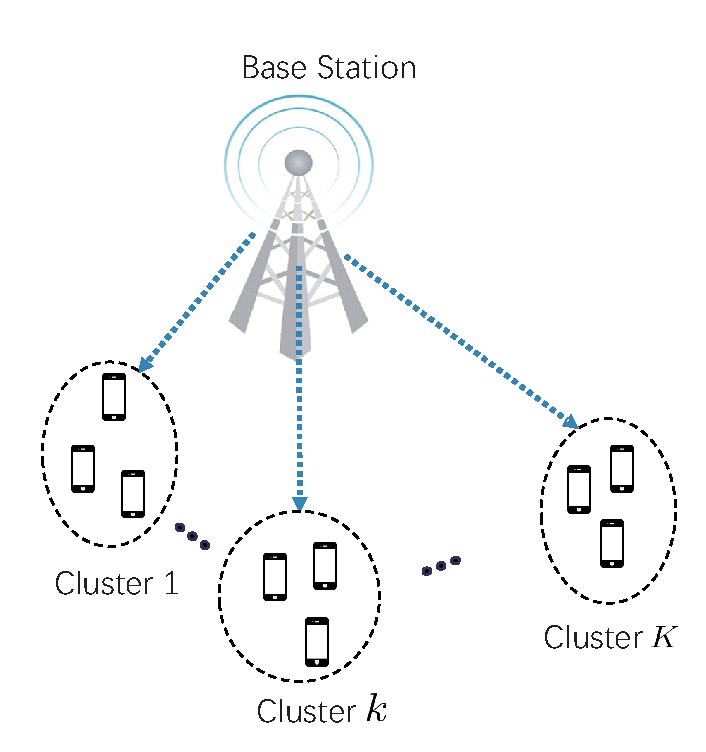
\includegraphics[scale=0.55]{PPTFigure/groupcluster.eps}
		\caption{Group scheduling to reduce the number of RF chains and eliminate the intra-cluster interference}\label{fig:BDMA}
	\end{center}
\end{figure}

{\color{red}However, the minimal number of RF chains is constrained by the transmitted data stream. In our proposed system, the users are grouped to several clusters and then communicate with base station in turn. We assume the symbol duration is much larger than time delay thus the received symbols of different users are same. Compared to serve each cluster separately, the interference will increase since each user has to decode received signal from other clusters. Thanks to the scheduling of users, we can firstly use analog precoding to eliminate the inter-cluster interference between cluster and then implement digital precoding to suppress the intra-cluster interference. The simulation results show that our proposed algorithm can efficiently reduce the number of RF chains without introducing large intra-cluster interference.} 

\underline{Notation}: Vectors and matrices are denoted by boldface letters. ${\bm A}^T$ and ${\bm A}^H$ denote transpose and conjugate transpose of ${\bm A}$, respectively. $\bm{A}^\dagger$ being the pseudo inverse of $\bm{A}$ while $||\bm{A}|| $ and $|\bm{A}|$ stand for the Frobenius norm and determinant of ${\bm A}$, respectively. $\bm{A}(i,j)$ denotes the $i$ row, $j$ column element of ${\bm A}$; $|\cal{I}|$ is the cardinality of the enclosed set ${\cal I}$; Finally, $\mathbb{E}[\cdot] $ and $\Re\{\cdot\}$ denote the expectation and real part of a random variable.

\begin{figure*}[htpb]
	\centering
	\begin{minipage}[t]{0.7\linewidth}
		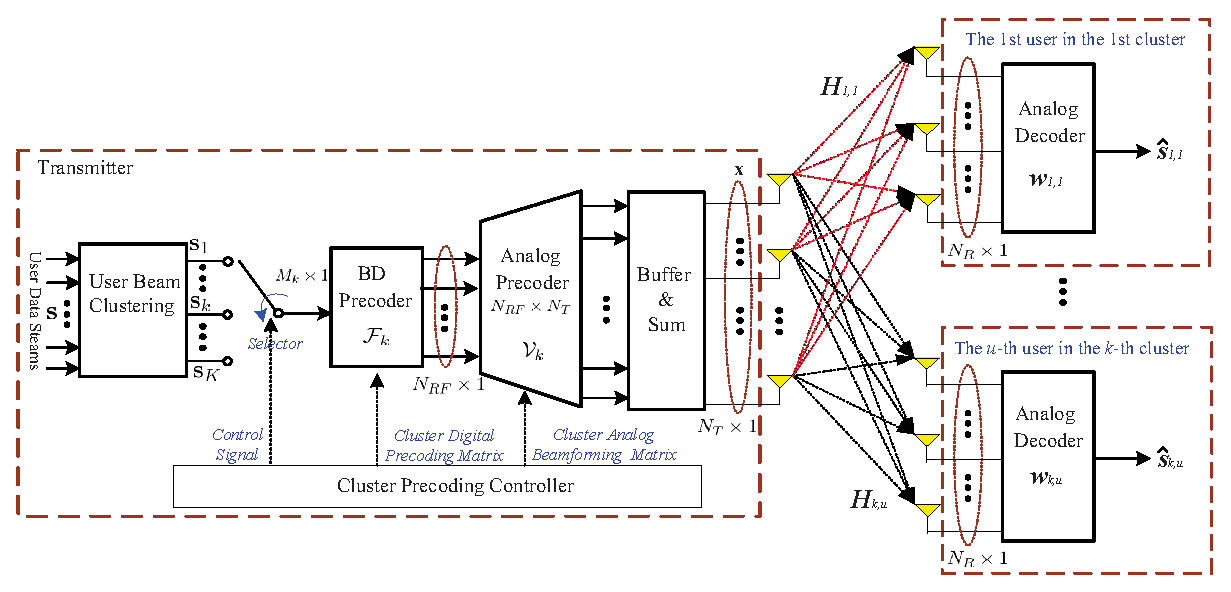
\includegraphics[width=5.6in,height=3in]{PPTFigure/BlockDiagonal.eps}
		\caption{Block diagram of the hybrid precoding system under consideration}\label{fig:BlockDiagram}
		\parbox{6.5cm}{\small \hspace{1.5cm} }
	\end{minipage}
\end{figure*}

\section{system model}
We consider a multi-user mmWave MIMO system shown in \figurename{ \ref{fig:BlockDiagram}}, in which a transmitter equipped with $N_{RF}$ RF chains and $N_T$ antennas transmits $N_U$ data streams to $N_U$ receivers with $N_R$ receive antennas. Following the same assumption commonly employed in the literature \cite{alkhateeb2015limited}, we assume only one data stream is designated to each scheduled receiver. We use ${\bm s}(n)$ to denote the $n$-th block of $N_U$ data to be transmitted with $\mathbb{E}\left[\bm{ss}^H\right]=\frac{1}{N_U}\bm{I}_{N_U}$. In the sequel, we concentrate on a single block and omit the temporal index $n$ for notational simplicity.


The hybrid precoding system first multiplies ${\bm s}$ with the digital precoding matrix $\bm{F}=\left[{\bm f}_1,\cdots,{\bm f}_u,\cdots{\bm f}_{N_U}\right]$ with ${\bm f}_u$ of dimension $N_{RF}\times 1$ being the digital beamforming vector for the $u$-th user, $u=1,2,\cdots,N_U$. After that, the output signal will be multiplied by the analog precoding matrix $\bm{V}=\left[{\bm v}_1,\cdots,{\bm v}_i,\cdots,{\bm v}_{N_{RF}}\right]$ with ${\bm v}_i$ of dimension $N_T\times 1$ being the $i$-th analog beamforming vector for $i=1,2,\cdots,N_{RF}$. The resulting precoded signal $\bm x$ of dimension $N_T\times 1$  can be expressed as

\begin{equation}{\label{eq:transx1}}
{\bm x} = \bm{V}\cdot \bm{F}\cdot\bm{s}= \bm{V}\sum_{u=1}^{N_U}\bm{f}_us_u
\end{equation}

The precoded signal $\bm x$ is then broadcast to $N_U$ users. The signal received by the $u$-th user is given by

\begin{eqnarray}{\label{eq:transx2}}
{\bm y}_u &=& \bm{H}_u \bm{x} + \bm{n}_u \nonumber\\
&=&\underbrace{\bm{H}_u \bm{V}\bm{f}_us_u}_\text{Desired Signal}+\underbrace{\bm{H}_u \bm{V}\sum_{\substack{i=1 \\ i\neq u}}^{N_U}\bm{f}_is_i}_\text{Interference}+\underbrace{\bm{n}_u}_\text{Noise},
\end{eqnarray}
where $\bm{H_u}$$\in\mathbb{C}^{N_R\times N_T}$ is the MIMO channel matrix between the transmitter and the $u$-th receiver\cite{el2014spatially}. Furthermore, $\bm{n}_u$ is complex additive white Gaussian noise with zero mean and variance equal to $\sigma^2$.

Assuming the receivers are all low-cost terminals that perform analog beamforming only in decoding, the decoded signal by the $u$-th user denoted by $\hat{s}_u$ is given by
\begin{equation}{\label{eq:hats}}
\hat{s}_u = \bm{w}_u^H \bm{H}_u \bm{V} \bm{f}_{u} \bm{s} + \bm{w}_u^H \bm{\tilde{n}}_u,
\end{equation}
where ${\bm w}_u$ of dimension $N_R\times 1$ is the analog beamforming vector employed by the $u$-th receiver with the power constraint of $|\bm{w}_u|^2=1$ and
\begin{equation}
\bm{\tilde{n}}_u=\bm{H}_u \bm{V}\sum_{\substack{i=1 \\ i\neq u}}^{N_U}\bm{f}_is_i+\bm{n}_u.
\end{equation}
Note that the first term in Eq.~(\ref{eq:hats}) stands for the desired signal while the second term is the sum of its own receiver noise and interference from other users.

\subsection{Channel Model}
As shown in \cite{rappaport2014millimeter}, the mmWave wireless channel can be well modeled by the Saleh-Valenzuela model. Following the same approach developed in \cite{alkhateeb2014channel}, we assume that each scatter only contributes one single propagation path. As a result, the $u$-th user's channel model can been modeled as:
\begin{equation}{\label{eq:Hu}}
\bm{H}_u = \sqrt{\frac{N_{T}N_{R}}{L_{u}}}\sum_{l=1}^{L_u}\alpha_{u,l}\cdot \bm{a}_{R}(\phi^r_{u,l},\theta^r_{u,l}) \cdot\bm{a}_{T}^{H}(\phi^t_{u,l},\theta^t_{u,l}),
\end{equation}
where $L_u$ is the number of scatters of the $u$-th user's channel. Furthermore, $\alpha_{u,l}$, $\theta^r_{u,l}/\phi^r_{u,l}$ and $\theta^t_{u,l}/\phi^t_{u,l}$ are the complex path gain, azimuth/elevation angles of arrival(AoA) and azimuth/elevation angles of departure(AoD) of the $l$-th path of the $u$-th user, respectively. Finally, ${\bm a}$ is the array response vector. For an uniform planar array (UPA) of size $P\times Q$ considered in this work, the array response vector ${\bm a}$ is given by \cite{alkhateeb2014channel}
\begin{flalign}\label{eq:UPAvec1}
\bm{a}(\phi,\theta) =&\frac{1}{\sqrt{N_T}}\left[1,  e^{jkd(\sin\phi \sin\theta +\cos\theta)},\cdots,\right.&&\nonumber\\
&\left. e^{jkd\left(p\sin\phi \sin\theta +q\cos\theta\right)},\cdots, \right. &&\nonumber\\
&\left. e^{jkd\left((P-1)\sin\phi \sin\theta +(Q-1)\cos\theta\right)}\right]^T,&&
\end{flalign}
where $k=\frac{2\pi}{\lambda}$ is the wavenumber while $d$ is the distance between two adjacent antennas.

%\subsection{Grouping for Users Under Base Station}
%For simplicity, the group users are divided uniformly and then the users under a base station can be divided into $K$ clusters with $N_K = N_U/K$ in each cluster. Thus, the digital precoder is given by
%\begin{equation}
%\bm{F} = 
%\begin{bmatrix}
%\bm{F}_{1}&\bm{F}_{2}&\cdots&\bm{F}_{K}\\
%\end{bmatrix}
%%\begin{bmatrix}
%%\bm{F}_{11}& \bm{F}_{12}&\cdots&\bm{F}_{1K}\\
%%\bm{F}_{21}& \bm{F}_{22}&\cdots&\bm{F}_{2K}\\
%%\cdots&\cdots&\cdots&\cdots\\
%%\bm{F}_{K1}&\bm{F}_{K2}&\cdots&\bm{F}_{KK}
%%\end{bmatrix}
%\end{equation}
%Where
%\begin{equation}
%\bm{F}_k =
%\begin{bmatrix}
%	\bm{f}_{11}&\bm{f}_{12}&\cdots&\bm{f}_{1N_K}
%\end{bmatrix}
%\end{equation}
%means the column vectors of digital precoder in $k$-th cluster.
%%The Eq. \eqref{eq:transx1} can be rewritten as 
%%\begin{eqnarray}{\label{eq:rewrite1}}
%%{\bm x} &=& [\bm{V}_1, \bm{V}_2, \cdots, \bm{V}_K]\cdot \bm{F}\cdot\bm{s} \nonumber\\
%%    	&=& \sum_{k=1}^{K}\sum_{i=1}^{K}\bm{V}_i \bm{F}_{ik} \bm{s}_k
%%\end{eqnarray}
%
%The signal received by $u$-th user in $k$-th cluster is given by 
%\begin{eqnarray}{\label{eq:rewrite2}}
%{\bm y}_{uk} &=&\underbrace{\bm{H}_u \bm{V}\bm{f}_{uk}{s}_{uk}}_\text{Desired Signal}+\underbrace{\bm{H}_u \bm{V}\sum_{\substack{i=1 \\ i\neq u}}^{N_K}\bm{f}_{ik}s_{ik}}_\text{Inner-cluster Interference} \nonumber\\
%&+& \underbrace{\bm{H}_u \bm{V}\sum_{j\neq k}^K \sum_{t=1}^{N_K} \bm{f}_{tj}{s}_{tj}}_\text{Intra-cluster Interference}+ \underbrace{\bm{n}_u}_\text{Noise}
%\end{eqnarray}
%
%where $s_uk$ is the $u$-th signal for $u$-th user in $k$-th cluster. Compared to Eq. \eqref{eq:transx2}, there is nothing special but the interference term is separated as inner-cluster and intra-cluster interference corresponding to the user scheduling.
\subsection{Problem Formulation}
For notational simplicity, we denote by ${\bm{g}}_{u}^H$ the effective array gain of the $u$-th user with
\begin{equation}\label{eq:defgu}
{\bm{g}}_{u}^H = \bm{w}^H_u \bm{H}_u \bm{V}.
\end{equation}

Then, the channel capacity of the $u$-th user is given by
\begin{equation}\label{eq:convenR}
R_u = \log\left(1+\frac{\frac{P}{N_U}|{\bm{g}}_{u}^H \bm{f}_u|^2}{\frac{P}{N_U}\displaystyle\sum_{\substack{i=1 \\ i\neq u}}^{N_U}|{\bm{g}}_{u}^H\bm{f}_i|^2+\sigma^2}\right).
\end{equation}
Subsequently, the system sum-rate capacity that is a function of ${\bm V}$ and ${\bm F}$ can be computed as
\begin{equation}
R_{tot}=\sum_{u=1}^{N_U}R_u.
\end{equation}

Finally, the optimal design of the digital and analog precoding matrices can be formulated as
\begin{align}\label{eq:maxsumrate}
\left\{{\bm V}^*,{\bm F}^*\right\} &= \argmax_{\tilde{\bm V},\tilde{\bm F}} R_{tot}\left(\tilde{\bm V},\tilde{\bm F}\right)\\ \nonumber
s.t. \quad&||\tilde{\bm V}\tilde{\bm f}_u||^2 = 1, \quad u=1,2,\cdots,N_U.
\end{align}

For the single-path LoS environment considered in previous work, the channel matrix of the $u$-th user is well structured as given by Eq.~\eqref{eq:HuLu1}. Subsequently, the optimal analog precoding at the transmitter is given by ${\bm v}^*_u = {\bm a}_T\left(\phi^t_u,\theta^t_u\right)$ while the optimal analog beamforming vector at the receiver is given by ${\bm w}^*_u = {\bm a}_R\left(\phi^r_u,\theta^r_u\right)$\cite{alkhateeb2014channel}. Assuming that the transmitter has perfect channel state information (CSI), then all AoA and AoD information, {\em i.e.} $\left\{\phi^t_u,\theta^t_u,\phi^r_u,\theta^r_u\right\}$, is perfectly known to the transmitter. As a result, the optimization problem in Eq.~(\ref{eq:maxsumrate}) can be simplified as
\begin{flalign}\label{eq:optdigPreMat}
{\bm F}^* &= \argmax_{\tilde{\bm F}} R_{tot}\left({\bm V}^*,\tilde{\bm F}\right)\\
s.t. \quad&||{\bm V}^*\tilde{\bm f}_u||^2 = 1 , \quad u=1,2,\cdots,N_U.\nonumber
\end{flalign}

We denote by $\hat{\bm s}=\left[\hat{s}_1,\hat{s}_2,\cdots,\hat{s}_{N_U}\right]^T$ the estimated signal vector. Recalling Eq.~(\ref{eq:hats}), $\hat{\bm s}$ can be expressed as \cite{alkhateeb2014channel}
\begin{equation}\label{eq:hatsAllUsers}
\hat{\bm s} = {\bm G}\cdot \bm{F} \cdot\bm{s} + \bm{\xi},
\end{equation}
where ${\bm G}=\left[{\bm g}_1,{\bm g}_2,\cdots,{\bm g}_{N_U}\right]^H$ is of dimension $N_U\times N_{RF}$ and ${\bm \xi}=\left[{\bm w}_1^H\tilde{\bm n}_1,{\bm w}_2^H\tilde{\bm n}_2,\cdots,{\bm w}_{N_U}^H\tilde{\bm n}_{N_U}\right]^T$. \cite{alkhateeb2014channel} proposed a zero-forcing approach to solve Eq.~(\ref{eq:optdigPreMat}) by setting
\begin{equation}\label{eq:ZFU-HBF}
\bm{F}_{ZF}={\bm G}^\dagger = \bm{G}^H(\bm{G}\bm{G}^H)^{-1},
\end{equation}
with $N_{RF}\geq N_U$.

To satisfy the power constraint, power normalization is performed on each ${\bm f}_u$ derived from $\bm{F}_{ZF}=\left[\bm{f}_{ZF,1},\bm{f}_{ZF,2},\cdots,\bm{f}_{ZF,N_U}\right]$ as
\begin{equation}\label{eq:ZFU-HBF}
\bm{f}^*_{ZF,u} = {\frac{\bm{f}_{ZF,u}}{||\bm{V}\cdot\bm{f}_{ZF,u}||}}.
\end{equation}

 

\section{Block Diagonal Digital Precoder}
\subsection{Single-path Channel Model}
We firstly consider the single-path case. Although the zero-forcing digital precoding has good performance on eliminating interference of users, the minimal number of required RF chains is limited by the number of data steams (is equal to the number of users). To overcome this problem, we design the block diagonal digital precoder to reduce the number of RF chains by writing the digital precoding matrix as
\begin{equation}\label{digitalblock}
	\bm{F} = diag(\bm{F}_1, \bm{F}_2, \cdots, \bm{F}_K)
\end{equation}
Where the users are divided into $K$ clusters and each cluster has $M_k$ users. The $\bm{F}_k\in \mathbb{C}^{M_k\times M_k}$ is the corresponding digital precoding matrix for each cluster. Thus, the number of RF chains can be reduced to $N_{RF} = \max(\{M_k\}_{k=1}^{K})$ 

Similarly, the analog precoding can be written as
\begin{equation}\label{analogblock}
	\bm{V} = [\bm{V}_1, \bm{V}_2, \dots, \bm{V}_K],\quad \bm{V}_k\in \mathbb{C}^{M_k\times M_k}
\end{equation}

By substituting Eq. \eqref{digitalblock} and \eqref{analogblock} to \eqref{eq:transx2},  the received signal of $u$-th user in $k$-th cluster can be represented as
\begin{eqnarray}{\label{eq:rewrite2}}
{\bm y}_{uk} &=&\underbrace{\bm{H}_{uk} \bm{V}_k\bm{f}_{uk}{s}_{uk}}_\text{Desired Signal}+\underbrace{\bm{H}_{uk} \bm{V}_k\sum_{\substack{i=1 \\ i\neq u}}^{M_K}\bm{f}_{ik}s_{ik}}_\text{Intra-cluster Interference} \nonumber\\
&+& \underbrace{\bm{H}_{uk}\sum_{\substack{j=1\\j\neq k}}^{K}\bm{V}_j\bm{F}_j\bm{s}_j }_\text{Inter-cluster Interference}+ \underbrace{\bm{n}_{uk}}_\text{Noise}
\end{eqnarray}
where $\bm{f}_{uk}$ is the $u$-th column vector in $\bm{F}_k$

With the assumption for infinite transmitter antennas in channel model Eq. \eqref{eq:Hu}
\begin{equation}
\lim_{N\rightarrow +\infty} \bm{a}^H_{T}(\phi^t_{i,l},\theta^t_{i,l}) \cdot\bm{a}_{T}(\phi^t_{j,p},\theta^t_{j,p})=\delta(i-j)\delta(l-p),
\end{equation}
and the single-path LoS channel model
\begin{equation}{\label{eq:HuLu1}}
\bm{H}_{uk} = \sqrt{N_{T}N_{R}}\cdot\alpha_u \cdot\bm{a}_{R}(\phi^r_{u},\theta^r_{u})\cdot\bm{a}^{H}_{T}(\phi^t_{u},\theta^t_{u}),
\end{equation}

the following deduction can be given
\begin{equation}\label{approx}
	\bm{H}_{uk}\bm{V}_{j} \approx 0 \quad \text{for} \quad k \neq j
\end{equation}

Then, the decoded signal can be rewritten as
\begin{equation}\label{Eq:receivedsignal}
	s_{uk} \approx \bm{g}_{uk}\bm{f}_{uk}s_{uk} + \bm{g}_{uk}\sum_{\substack{i=1\\i\neq u}}^{M_k}\bm{f}_{ik}s_{ik}+\bm{w}_{uk}\bm{n}_{uk}
\end{equation}
Where $\bm{g}_{uk} = \bm{w}_{uk}\bm{H}_{uk}\bm{V}_k$ is the corresponding effective array gain of $u$-th user in $k$-th cluster.


Then, the channel capacity of the $u$-th user in $k$-th cluster is given by 
\begin{equation}\label{eq:6}
R_{uk} = \log\left(\frac{\frac{P}{N_U}|\bm{g}^H_{uk}\bm{f}_{uk}|^2}{\frac{P}{N_U}\left(\displaystyle\sum_{\substack{i=1 \\ i\neq u}}^{M_k}|{\bm{g}}_{uk}^H\bm{f}_{ik}|^2\right)+\sigma^2}+1\right)
\end{equation}
Finally, the system sum-rate capacity that is a function of ${\bm V}_k$ and ${\bm F}_k$ can be computed as
\begin{equation}
R_{tot}=\sum_{k=1}^{K}\sum_{u=1}^{M_k}R_{uk}.
\end{equation}

To minimize the inner-cluster interference, the group scheduling problem is formulated as
\begin{align}\label{eq:group-scheduling}
\{\bm{V}_k\}_{k=1}^{K} &= \argmax \frac{||\bm{w}_{uk} \bm{H}_{uk} \bm{V}_k||_F^2}{\sum_{i=1,i\neq k}^{N_U}||\bm{w}_{uk} \bm{H}_{uk} \bm{V}_i||_F^2}  \\ \nonumber
s.t. &\quad \bm{V}_{k} \in  \{\bm{v_u}\}_{u=1}^{N_U} \quad k = 1,2,\cdots,K
\end{align}
And the corresponding digital precoder can be solved by $K$ subproblems as shown in Eq. \eqref{eq:optdigPreMat}. There is noting special but $\bm{V}$ and $\bm{F}$ are replaced by $\bm{V}_k$ and $\bm{F}_k$.




\subsection{Multi-path Channel Model}
For multi-path channel model as shown in Eq. \eqref{eq:Hu}, the only difference is that the channel model is represented as the summation of multiple single-path. We need to select the beams with least interference. Based on the idea of BDMA, the analog precoder is solved by

\begin{align}\label{eq:analogprecoder}
\{\bm{v}_u\}_{u=1}^{N_U} &= \argmax \frac{||\bm{w}_u \bm{H}_u \bm{v}_u||_F^2}{\sum_{i=1,i\neq u}^{N_U}||\bm{w}_u \bm{H}_u \bm{v}_i||_F^2}  \\ \nonumber
s.t. &\quad \bm{v}_u \in \{ \bm{a}_{T}(\phi^t_{u,l},\theta^t_{u,l})\}_{l=1}^{L_u}
\end{align}

After obtained the analog precoder, the problem can be simplified as group-scheduling problem of single-path channel model and can be solved by Eq. \eqref{eq:group-scheduling} and \eqref{eq:optdigPreMat}.


%\subsection{Convex Optimization}
%Another method to realize the block diagonal matrix is minimizing the interference between ZFU-HBF and block-diagonal digital precoding by convex optimization. The convex problem is formulated as
%\begin{align}
%	\bm{F}^*_{Block} &= \argmin ||\bm{GF}_{ZF} - \bm{G} \bm{F}_{Block}||_F^2 \\
%	s.t. &\quad [\bm{F}_{Block}]_{ij} =0 \quad \text{for} \quad j \neq k, j\in (1,K) \nonumber
%\end{align}
\subsection{Greedy group scheduling algorithm}
Although we can get the global optimal solution of group scheduling problem by exhaustive searching, the computational cost is also very huge. Compared with fully zero-forcing algorithm, the more block we use, the  larger residual interference will be imported since the Eq. \eqref{approx}.

The algorithm can be summarized as Algorithm \ref{selection}.
\begin{algorithm}[h] 		
	\caption{Greedy scheduling algorithm for PAPR-aware hybrid beamforming}
	\label{selection}
	\begin{algorithmic}
		\REQUIRE  \quad
		\STATE	All user index set: $\mathcal{X}$\\
		\STATE  Selected user index set : $\mathcal{I}_k=\emptyset$, $k=1,2,\cdots, K$\\
		\STATE  Number of clusters: $K$\\
		\STATE  Analog precoder solved by Eq. \eqref{eq:analogprecoder}: $\bm{V}=[\bm{v}_1,\bm{v}_2,\cdots,\bm{v}_{N_U}]$
		\ENSURE   	
		\STATE Initialization: Assign the user index $x$ corresponding to the largest channel gain $|\alpha|$ to ${\mathcal I}_1$, {\em i.e.} $\mathcal{I}_1 \leftarrow  x$ and ${\mathcal X}\setminus x$, 
		\STATE $\bm{V}_{else} = [v_1]$
		\FOR{$x$ in $\mathcal{x}$}
		\STATE $p(x) = $
		\ENDFOR
		\WHILE{$|{\cal I}|< N_U$}
		\STATE ${\bm A}=\left[\bm{a}_{T}\left(\phi^t_{i_1},\theta^t_{i_1}\right),\bm{a}_{T}\left(\phi^t_{i_2},\theta^t_{i_2}\right),\cdots,\bm{a}_{T}\left(\phi^t_{i_{|{\cal I}|}},\theta^t_{i_{|{\cal I}|}}\right)\right]$
		\STATE Compute the projection space: ${\bm P}_A = {\bm A}{\bm A}^{\dagger}$ 		 				
		\FOR{$x$ in {$\mathcal{X}$}}
		\STATE $p(x) = \|{\bm P}_A\cdot {\bm a}_T\left(\phi^t_{x},\theta^t_{x}\right)\|^2$ 				 								
		\ENDFOR
		\STATE  Find the user index $x^*$ with the minimum $p(x)$ 									
		\STATE	Update ${\cal I} \leftarrow  x^*$ and ${\cal X}\setminus x^*$	
		\ENDWHILE	
	\end{algorithmic}
\end{algorithm}

\section{Power Allocation for SIR}
In this section, we will discuss the power allocation of multi-user MIMO system. For high signal-to-noise(SNR) ratio scenario, the noise can be ignored. The powers for users are represented as $\bm{p}=[p_1, p_2, \cdots, p_{N_U}]$. 

The SIR of $u$-th user is set to be 
\begin{align}
	\gamma_u &= \frac{p_u|\bm{g}_u^H\bm{f}^*_{ZF,u}|^2}{\sum_{i\neq u}^{N_U}p_i|\bm{g}_u^H \bm{f}^*_{ZF,i}|^2} \nonumber\\
		     &= \frac{p_u|\bm{g}_u^H\bm{f}^*_{ZF,u}|^2}{\sum_{i=1}^{N_U}p_i|\bm{g}_u^H \bm{f}^*_{ZF,i}|^2 - p_u|\bm{g}_u^H \bm{f}^*_{ZF,u}|^2}
\end{align}

Considering the balanced SIR theory 
\begin{equation}
\gamma_u=\gamma, u=1,2,\cdots,N_U
\end{equation}

the transmitted power can be minimized by eigenvalue problem
\begin{equation}
	\bm{Gp} = \frac{\gamma+1}{\gamma} \bm{p}
\end{equation}
where 
\begin{equation}
\bm{G}=
\begin{bmatrix}
1&T_2/T_1&\cdots&T_{N_U}/T_1\\
T_1/T_2&1&\cdots&T_{N_U}/T_2\\
\cdots&\cdots&\cdots&\cdots\\
T_1/T_{N_U}&T_2/T_{N_U}&\cdots&1
\end{bmatrix}
\end{equation}
and
\begin{equation}
T_u = |\bm{g}_u^H \bm{f}^*_{ZF,u}|^2
\end{equation}
This problem can be easily solved by 
\begin{equation}
	\gamma = \frac{1}{\lambda_{max}(\bm{G})-1}
\end{equation}

As the elements of $\bm{G}$ are positive, from the \textit{Perron Frobenius Theorem}, we know there must exist at least one positive eigenvector and thus the power is solved.



\bibliography{BDMAref}
\bibliographystyle{IEEEtran}


% references section

\end{document}


